
\documentclass{ol-softwaremanual}
\usepackage{graphicx}  % for including images
\usepackage{microtype} % for typographical enhancements
\usepackage{minted}    % for code listings
\usepackage{amsmath}   % for equations and mathematics
\setminted{style=friendly,fontsize=\small}
\renewcommand{\listoflistingscaption}{List of Code Listings}
\usepackage{hyperref}  % for hyperlinks
\usepackage[a4paper,top=4.2cm,bottom=4.2cm,left=3.5cm,right=3.5cm]{geometry} % for setting page size and margins

\graphicspath{ {./images/} }

% Custom macros used in this example document
\newcommand{\doclink}[2]{\href{#1}{#2}\footnote{\url{#1}}}
\newcommand{\cs}[1]{\texttt{\textbackslash #1}}
% \definecolor{plantucolor0000}{RGB}{255,255,255}
% \definecolor{plantucolor0001}{RGB}{24,24,24}
% \definecolor{plantucolor0002}{RGB}{0,0,0}
% \definecolor{plantucolor0003}{RGB}{226,226,240}
% \definecolor{plantucolor0004}{RGB}{238,238,238}
% Frontmatter data; appears on title page
\title{Technical Document \\Template}
\version{2.3.1}
\author{Overleaf}
% \softwarelogo{
\includegraphics[width=8cm]{logo}}



\begin{document}

\maketitle

\tableofcontents
\listoflistings
\newpage

\section{Architecture}

\section{\mintinline{bash}|DEV| and \mintinline{bash}|TEST| environment}
\begin{figure}
    \centering
    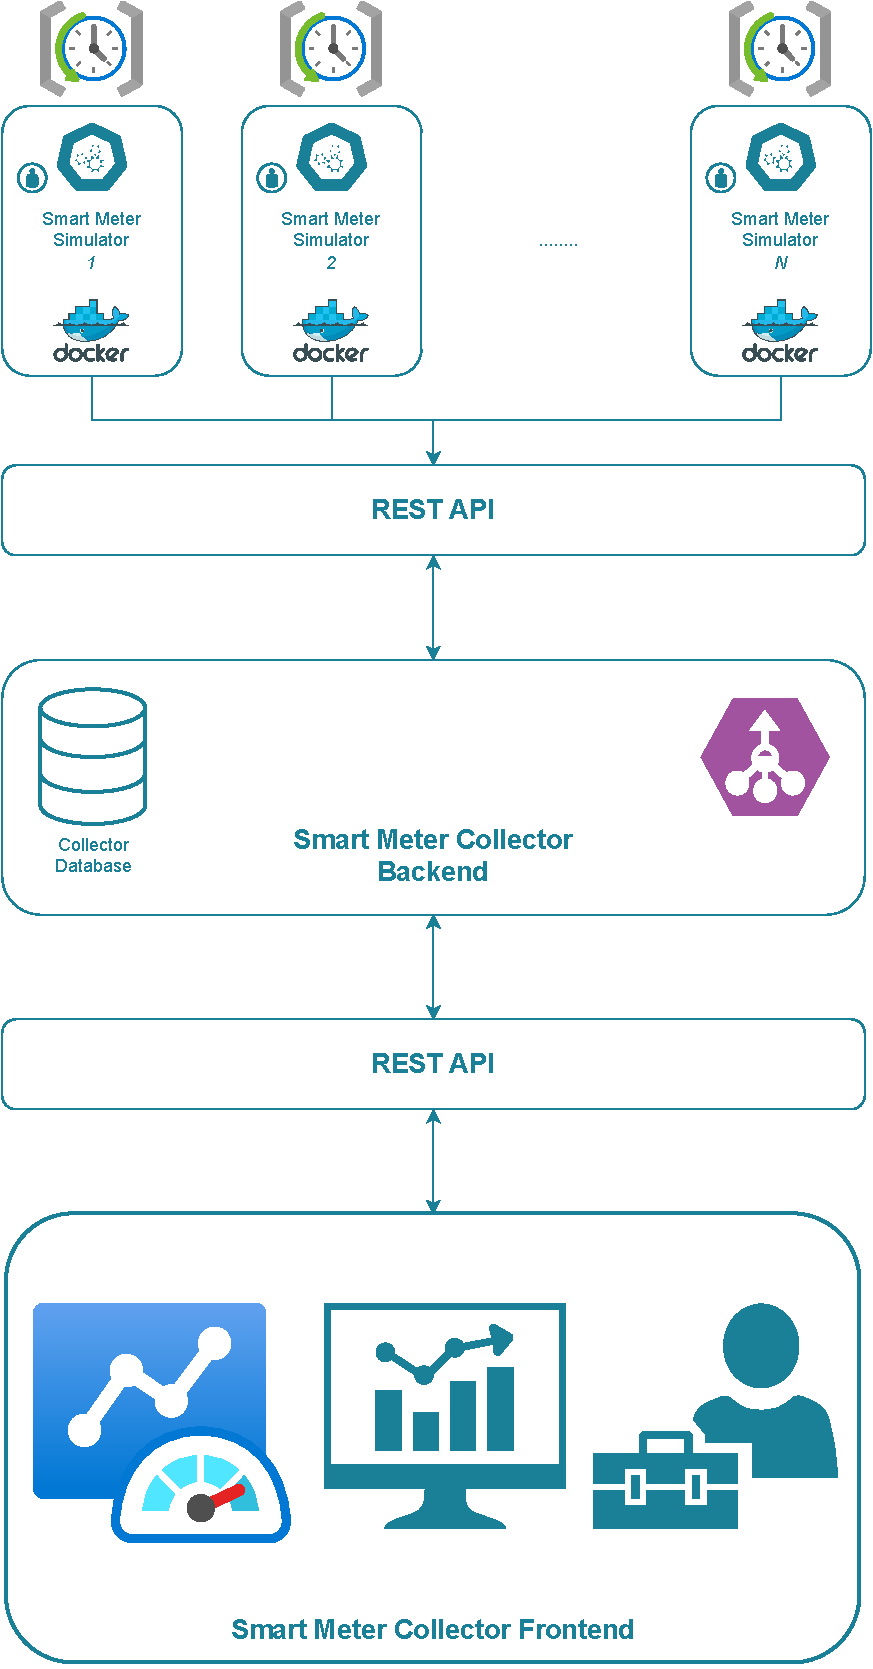
\includegraphics[width=0.7\textwidth]{fig_01}
    \caption{System Architecture}\label{fig::001}
\end{figure}


\section{Roles}
\noindent \textbf{Smart Meter (SM).} IoT device used to collect data about electrical energy consumption or production in particular household. In development and testing environment SM is replaced by Smart Meter Simulator (SMS) which is implemented by runnable docker containers. SM(S) comes with the following functionalities:
\begin{itemize}
    \item register to SMCB,
    \item send data to SMBC,
    \item re-send data to SMBC in case of failure.
\end{itemize}
\noindent \textbf{Smart Meter Collector Backend (SMCB).} The backend Flask application used to collect data from Smart Meter Simulators. This application qccepts 
\noindent \textbf{Client.} Application used by Smart Meter Simulator (SMS) to communicate with the Smart Meter Collector Backend.

The microservice architecture of the system in \mintinline{bash}|DEV| and \mintinline{bash}|TEST| environments is given in Figure \ref{fig::001}. Each smart meter is simulated by docker container instance that sends energy production/consumption data to Smart Meter Collector Backend. This communication is performed using Smart Meter Collector REST API (SMC REST API). Smart Meter Simulator (SMS) authenticates using OAuth 2.0 device authorization grant flow (\href{https://www.rfc-editor.org/rfc/rfc8628}{RFC8628}). This is a usual standard for authorization of input-constrained IoT devices where the authorization requested is authorized by end users on a separate device. Smart Meter Simulator requests access token using device authorization grant flow on initial running. User has to re-authorize devoce 

\subsection{Security standards}
\begin{itemize}
    \item rate limit to block user code brute forcing,
    \item lifetime of the code,
    \item high entropy 128-bit symmetric keys should be used.
\end{itemize}
\begin{itemize}
    \item register,
    \item send.
\end{itemize}


\begin{figure}
    \centering
    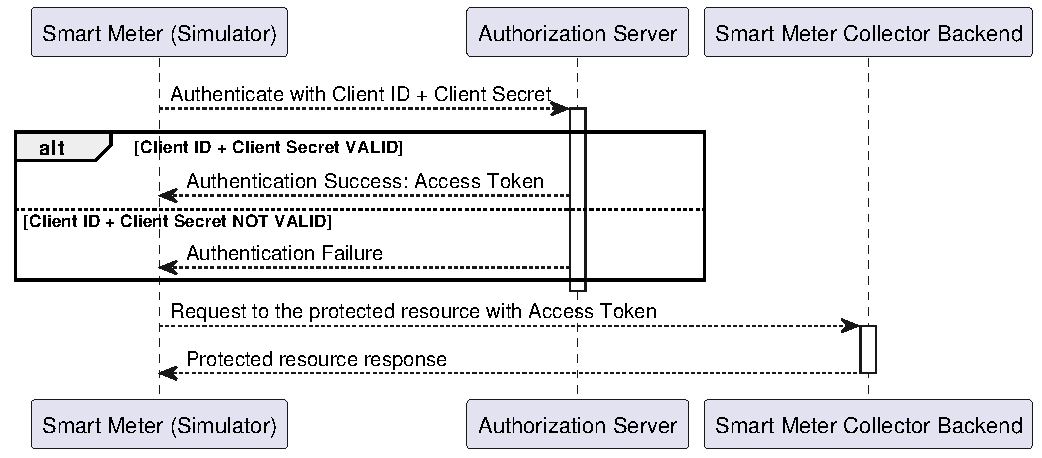
\includegraphics[width=0.9\textwidth]{fig_02}
    \caption{Client Credential Authorization Flow}\label{fig::002}
\end{figure}

\section{Including code samples}

%\input{code-samples}

\section{Some further examples to get started}

%\input{further-examples}

\end{document}
